\documentclass{beamer}

\usetheme{metropolis}

% Paquetes obligatorios
\usepackage{amsmath}
\usepackage{amssymb}
\usepackage{booktabs}
\usepackage{graphicx}
\usepackage{hyperref}
\usepackage{tikz}
\usepackage[spanish]{babel}
\usepackage{subcaption}

% Colores corporativos UDC
\definecolor{udcpink}{RGB}{177,0,114}
\definecolor{udcgray}{RGB}{100,100,100}

% Personalización metropolis con colores oscuros
\setbeamercolor{frametitle}{bg=udcpink!90!black, fg=white}
\setbeamercolor{progress bar}{fg=udcpink}
\setbeamercolor{alerted text}{fg=udcpink}

%----------------------------------------------------------------------------------------
%	TÍTULO
%----------------------------------------------------------------------------------------

\title[NIC]{Neural Image Compression (NIC): El fin de la era JPEG}
\subtitle{Compresión Neuronal de Imágenes}
\author[IGM]{
Daniel Quintillán Quintillán \\
Ponente 2 \\
Ponente 3 \\
Ponente 4 \\
Ponente 5
}
\institute[UDC]{
Introducción á Xestión Multimedia \\
Universidade da Coruña
}
\date{Mayo 2026}

\begin{document}

% Portada
\begin{frame}
\centering
\vspace{10pt}

\includegraphics[scale=0.2]{images/udc}
\titlepage
\end{frame}

% Índice
\begin{frame}{Índice}
\tableofcontents
\end{frame}

% Contenido por bloques
\section{El Problema y Cambio de Paradigma}

% --- Ponente 1 ---

\begin{frame}{El límite del diseño humano (\textit{Handcrafted})}
\begin{alertblock}{Internet colapsa bajo el peso visual}
El 80\% del tráfico de Internet es contenido visual (imágenes y vídeo).
\end{alertblock}
\begin{itemize}
    \item Los códecs clásicos (JPEG, HEVC) se basan en la \textbf{DCT} y procesamiento por bloques.
    \item Diseñados manualmente hace décadas, han alcanzado su \textbf{techo matemático}.
    \item Resultado: \textbf{artefactos de bloque} visibles a tasas bajas de bits.
    \item No aprovechan la redundancia semántica de la imagen.
\end{itemize}
\end{frame}

\begin{frame}{El Paradigma del Aprendizaje (NIC)}
\begin{block}{Neural Image Compression}
Dejar que una \textbf{red neuronal profunda} aprenda automáticamente la representación más eficiente de la imagen, sin reglas diseñadas a mano.
\end{block}
\vspace{0.5cm}
\textbf{Pregunta clave:}
\begin{enumerate}
    \item ¿Es \textbf{técnicamente} viable sustituir a JPEG hoy?
    \item ¿Es \textbf{industrialmente} viable su despliegue a escala?
\end{enumerate}
\end{frame}

\section{Fundamentos Técnicos}

% --- Ponente 2 ---

\begin{frame}{El Autoencoder Variacional (VAE)}
 \begin{figure}
     \centering
     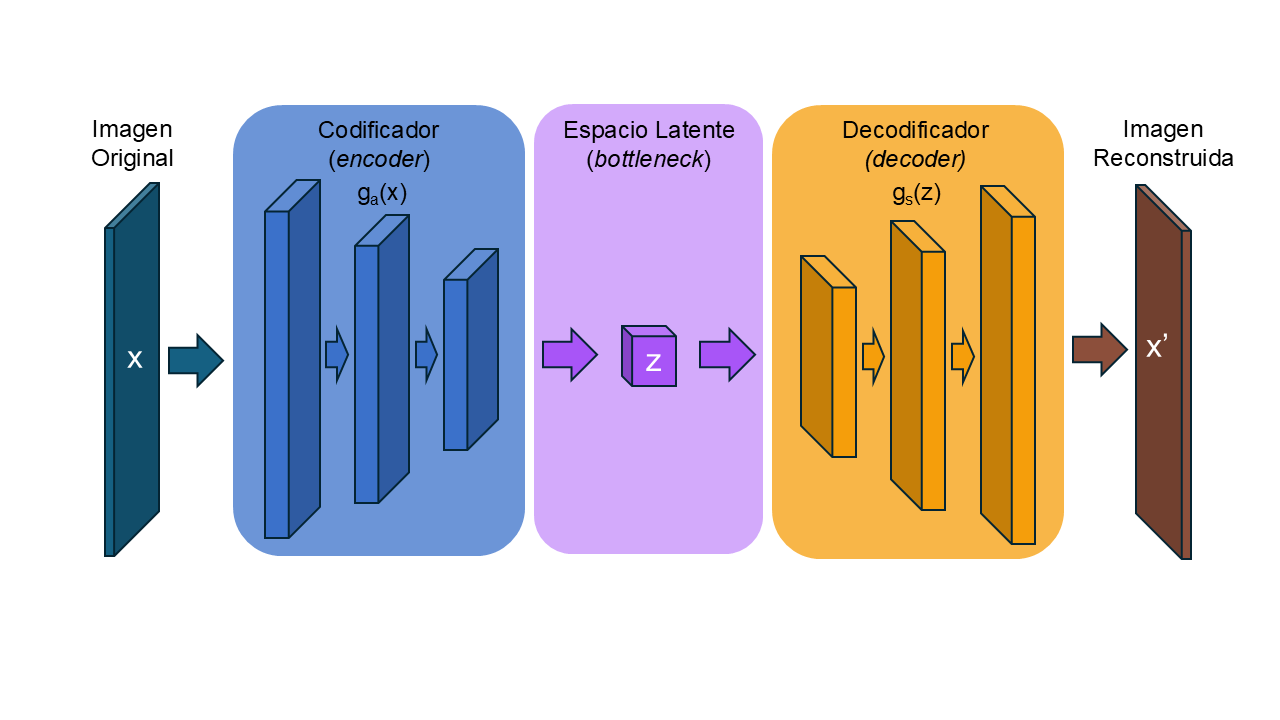
\includegraphics[width=0.9\textwidth]{images/diagrama_autoencoder}
     \caption{Arquitectura del Autoencoder Variacional para NIC.}
 \end{figure}
\end{frame}

\begin{frame}{El Compromiso Tasa-Distorsión}
\begin{alertblock}{Función de pérdida fundamental}
$$L = R + \lambda \cdot D$$
\end{alertblock}
\begin{itemize}
    \item $R$ (\textit{Rate}): Número de bits necesarios para codificar la representación latente.
    \item $D$ (\textit{Distortion}): Error de reconstrucción (calidad perdida).
    \item $\lambda$: Parámetro que \textbf{equilibra} compresión vs. calidad.
\end{itemize}
\vspace{0.3cm}
Un $\lambda$ alto prioriza calidad; un $\lambda$ bajo prioriza compresión.
\end{frame}

\begin{frame}{El Reto de la Cuantización}
\begin{itemize}
    \item La cuantización (redondeo a enteros) es \textbf{necesaria} para obtener un bitstream discreto.
    \item Problema: crea una función escalera con \textbf{gradiente nulo} $\rightarrow$ rompe la retropropagación.
\end{itemize}
\begin{exampleblock}{Solución: Ruido uniforme aditivo}
Durante el entrenamiento, se sustituye el redondeo por \textbf{inyección de ruido uniforme} $\mathcal{U}(-0.5, 0.5)$, creando un sustituto diferenciable.
\end{exampleblock}
\begin{itemize}
    \item En inferencia se usa el redondeo real.
    \item Permite entrenar el sistema end-to-end con descenso de gradiente.
\end{itemize}
\end{frame}

\section{Evolución y Resultados}

% --- Ponente 3 ---

\begin{frame}{Evolución Arquitectónica}
\begin{itemize}
    \item \textbf{Primera generación:} CNNs --- capturan patrones \textit{locales} eficientemente.
    \item \textbf{Segunda generación:} \textbf{Vision Transformers (ViT)} --- entienden el \textit{contexto global} mediante mecanismos de \textbf{atención}.
    \item La atención permite ponderar regiones distantes de la imagen para una codificación más eficiente.
\end{itemize}

% INSERTAR FIGURA 2 AQUI
% \begin{figure}
%     \centering
%     \includegraphics[width=0.8\textwidth]{images/evolucion_arquitecturas}
%     \caption{De CNNs a Vision Transformers en compresión neuronal.}
% \end{figure}
\end{frame}

\begin{frame}{Resultados vs. JPEG}
\begin{alertblock}{BD-Rate: 65\% de ahorro}
Los modelos NIC actuales ahorran un \textbf{65\% de bits} respecto a JPEG manteniendo la misma calidad visual en el dataset Kodak.
\end{alertblock}
\begin{itemize}
    \item Métrica \textbf{BD-Rate}: mide el ahorro porcentual de bits a calidad equivalente.
    \item Superan también a HEVC/Intra en múltiples benchmarks.
    \item Rendimiento consistente en distintos tipos de contenido.
\end{itemize}

% INSERTAR FIGURA 4 AQUI (Curva R-D)
% \begin{figure}
%     \centering
%     \includegraphics[width=0.8\textwidth]{images/curva_rd}
%     \caption{Curva Tasa-Distorsión: NIC vs. códecs clásicos.}
% \end{figure}
\end{frame}

\begin{frame}{Ventajas Perceptivas y Adaptabilidad}
\begin{itemize}
    \item \textbf{Fine-tuning} para dominios específicos:
    \begin{itemize}
        \item Radiografías médicas.
        \item Imágenes satelitales.
        \item Contenido artístico.
    \end{itemize}
    \item Uso de métricas perceptuales como \textbf{MS-SSIM} para optimizar para el ojo humano.
    \item Degradación \textbf{suave y gradual}, sin artefactos de bloque.
\end{itemize}

% INSERTAR FIGURA 5 AQUI
% \begin{figure}
%     \centering
%     \includegraphics[width=0.8\textwidth]{images/comparacion_perceptual}
%     \caption{Comparación perceptual: NIC vs. JPEG a misma tasa de bits.}
% \end{figure}
\end{frame}

\section{Retos y Casos de Uso}

% --- Ponente 4 ---

\begin{frame}{El Cuello de Botella del Hardware}
\begin{itemize}
    \item Modelos autorregresivos: tardan \textbf{segundos por imagen} en una CPU convencional.
    \item Complejidad computacional $\gg$ decodificadores JPEG.
    \item \textbf{Necesidad absoluta} de hardware dedicado:
    \begin{itemize}
        \item NPU (Neural Processing Unit).
        \item GPU con soporte de inferencia optimizada.
        \item Aceleradores ASIC específicos.
    \end{itemize}
\end{itemize}
\begin{alertblock}{Barrera de adopción}
Sin aceleración hardware, NIC no es viable para decodificación en tiempo real.
\end{alertblock}
\end{frame}

\begin{frame}{Casos de Uso Reales Actuales}
\begin{exampleblock}{Almacenamiento WORM en la nube}
Netflix / Meta: codifican una vez, leen millones de veces. El coste de codificación se amortiza masivamente.
\end{exampleblock}
\begin{itemize}
    \item \textbf{VCM} (Video Coding for Machines):
    \begin{itemize}
        \item Compresión optimizada para visión artificial.
        \item Coches autónomos, vigilancia, drones.
        \item La máquina no necesita ``calidad visual humana''.
    \end{itemize}
    \item Archivos digitales de larga duración.
    \item Streaming adaptativo con decodificación en servidor.
\end{itemize}
\end{frame}

\begin{frame}{Limitaciones Críticas: Alucinaciones Generativas}
\begin{alertblock}{Peligro: contenido inventado}
A tasas de bits extremadamente bajas, los modelos generativos \textbf{inventan texturas realistas pero falsas} (``alucinaciones'').
\end{alertblock}
\begin{itemize}
    \item La imagen reconstruida \textit{parece} correcta, pero contiene detalles ficticios.
    \item \textbf{Inasumible} en dominios críticos:
    \begin{itemize}
        \item Imágenes médicas (diagnóstico erróneo).
        \item Evidencia forense (pruebas judiciales).
        \item Cartografía y teledetección.
    \end{itemize}
    \item Requiere métricas de fidelidad estrictas, no solo perceptuales.
\end{itemize}
\end{frame}

\section{Impacto, Futuro y Conclusiones}

% --- Ponente 5 ---

\begin{frame}{Ecosistema y Estándar JPEG AI}
\begin{block}{ISO/IEC 6048-1 --- JPEG AI}
Primer estándar de compresión de imagen basado en redes neuronales, \textbf{libre de regalías}.
\end{block}
\begin{itemize}
    \item Adopción en silicio:
    \begin{itemize}
        \item Apple Neural Engine.
        \item Qualcomm Hexagon NPU.
        \item MediaTek APU.
    \end{itemize}
    \item Integración con \textbf{C2PA / JPEG Trust}:
    \begin{itemize}
        \item Autenticidad y procedencia de contenido.
        \item Defensa contra Deepfakes.
        \item Cadena de custodia criptográfica.
    \end{itemize}
\end{itemize}
\end{frame}

\begin{frame}{Conclusión: Despliegue ``Core-to-Edge''}
\begin{exampleblock}{Transición en 4 fases}
\begin{enumerate}
    \item \textbf{Servidores Cloud:} Codificación masiva offline (ya activo).
    \item \textbf{Apps Profesionales:} Edición, archivo, postproducción.
    \item \textbf{Smartphones con NPU:} Captura y compresión en dispositivo.
    \item \textbf{Reemplazo universal:} NIC como formato por defecto.
\end{enumerate}
\end{exampleblock}
\vspace{0.3cm}
\begin{itemize}
    \item La pregunta no es \textit{si} NIC reemplazará a JPEG, sino \textit{cuándo}.
    \item El estándar JPEG AI marca el inicio de la transición industrial.
\end{itemize}
\end{frame}


% Cierre
\begin{frame}[standout]
¡Gracias por su atención!
\end{frame}

\end{document}
